\documentclass[../main.tex]{subfiles}

\begin{document}

\newpage

\section{QCD}%
\label{sec:qcd}

\subsection{Sterke interactie}%
\label{sub:sterke_interactie}

\begin{figure}[h]
    \centering
    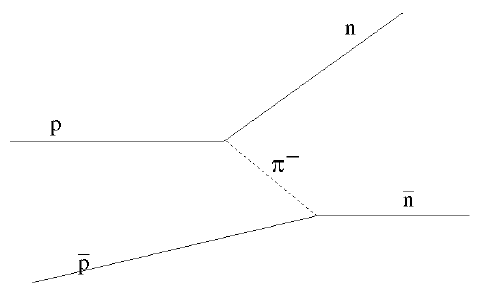
\includegraphics[width=0.6\linewidth]{QCD/ppnn.png}
    \caption{omvorming van protonen in neutronen}%
    \label{fig:ppnn}
\end{figure}

Historisch gezien is de sterke interactie ingevoerd om $p\overline p \rightarrow n\overline n$ te beschrijven. Hierbij werd gezegd dat deze nucleonen op vlak van kernkrachten gelijk zijn en een sterk isospin doublet vormen.
\begin{equation}
    \begin{aligned}
        \label{eq:nucleon_doublet}
        \begin{pmatrix}
            p\\
            n
        \end{pmatrix}
        \text{: sterk isospin doublet}
    \end{aligned}
\end{equation}
Dit is een SU(2) groep en heeft 3 generatoren en uitwisselingsdeeltjes
\begin{equation}
    \begin{aligned}
        \label{eq:isospin_uitwisseling_deeltjes}
        \begin{pmatrix}
            \pi^+\\
            \pi^0\\
            \pi^-
        \end{pmatrix}
    \end{aligned}
\end{equation}
Dit werkt redelijk, maar nu weten we natuurlijk dat dit niet correct is. Het grote probleem is dat deze uitwisselingsdeeltjes geen puntdeeltjes zijn, wat tot technische problemen zal leiden. Normaal verwachten we ook dat bij deze sterke wisseling een vectorboson het intermediair deeltje zou zijn met spin 1. De spin van de pionen is niet 1, maar 0, wat een groot probleem is. De reden waarom we weten dat we een spin 1 deeltje nodig hebben als intermediair deeltje, kunnen we halen uit het deuterium dat we eerder besproken hebben. We hebben gezien dat er tussen het spin triplet en singlet een energieverschil zit en de spin wel degelijk zal uitmaken bij deze sterke interactie. We moeten dus gaan zoeken naar meer detail. Dit is dan uiteraard vervangen door het beeld dat we nu hebben met het proton en neutron bestaande uit quarks en deze quarks die dan interageren met elkaar met behulp van gluonen.

\subsubsection{@ Quark level}%
\label{ssub:_quark_level}

Als we bij steeds hogere energie deze sterke interacties onderzoeken, moeten we meer en meer rekening beginnen houden met de individuele bijdrages van de quarks. Bij deze hogere energieën kwam er nog een ander probleem naar boven dat kon gezien worden aan de hand van $\Delta^{++}=\left|u^\uparrow u^\uparrow u^\uparrow\right>$. We zien dat deze golffunctie volledig symmetrisch is:
\begin{itemize}
    \item Spatiaal: $l=0$
    \item Flavour: allemaal $u$ quarks
    \item Spin: zijn allemaal naar omhoog gericht
\end{itemize}
wat tot dan totaal niet kon volgens Pauli. Om dit op te lossen wordt een nieuw kwantumgetal toegevoegd in de $SU(3)$ groep, kleur. Dit is het ontstaan van QCD. We zorgen dat de golffunctie van de kleur volledig antisymmetrisch is. De 3 nieuwe ladingen voor de kleur zijn
\begin{equation}
    \begin{aligned}
        \label{eq:kleur_lading}
        \begin{pmatrix}
            r\\
            g\\
            b
        \end{pmatrix}
    \end{aligned}
\end{equation}
Omdat we $SU(3)$ hebben, hebben we 8 generatoren wat neerkomt op 8 uitwisselingsdeeltjes.

\subsection{Symmetrie van de sterke wisselwerking}%
\label{sub:symmetrie_van_de_sterke_wisselwerking}

Het bewijzen dat er juist 3 kleurladingen zijn gebeurt als volgt. We kijken naar de verhouding van de werkzame doorsnedes van $e^+e^-$ verval naar hadronen en muonen.
\begin{equation}
    \begin{aligned}
        \label{eq:experiment_sterke_sym}
        R(\sqrt{s}) &= \frac{\sigma(e^+e^- \rightarrow \text{hadrons})}{\sigma(e^+e^- \rightarrow \mu^+\mu^-)}\\
                    &= \frac{\sum_c\sum_q \int \left|
                        \feynmandiagram[inline=(a), horizontal=a to b]{
                        a -- [photon, edge label=\(\gamma\)] b,
                        i1 [particle=\(e^-\)] -- [fermion] a,
                        a -- [fermion] i2 [particle=\(e^+\)],
                        f1 [particle=\(q'\)] -- [fermion] b,
                        b -- [fermion] f2 [particle=\(q\)],
                    };
                    \right|^2}{\int \left|
                    \feynmandiagram[inline=(a), horizontal=a to b]{
                        a -- [photon, edge label=\(\gamma\)] b,
                        i1 [particle=\(e^-\)] -- [fermion] a,
                        a -- [fermion] i2 [particle=\(e^+\)],
                        f1 [particle=\(\mu^+\)] -- [fermion] b,
                        b -- [fermion] f2 [particle=\(\mu^-\)],
                    };
                    \right|^2}\\
                    &= N_c\sum_q Q_q^2
    \end{aligned}
\end{equation}
Het enige verschil tussen de 2 diagrammen naast de massa van de deeltjes is het ladingsverschil tussen de uitgaande deeltjes. We kunnen dus het aantal kleuren letterlijk waarnemen.

\begin{figure}[h]
    \centering
    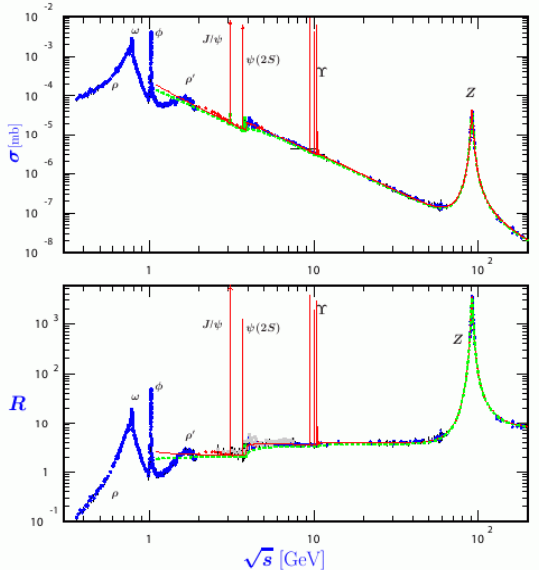
\includegraphics[width=0.8\linewidth]{QCD/ee_scattering.png}
    \caption{De resultaten van verschillende $e^+e^-$ verstrooiingen}%
    \label{fig:ee_scattering}
\end{figure}

Indien het foton maar juist genoeg energie heeft om een specifiek quark-antiquark paar aan te maken zullen deze niet van elkaar weg bewegen en krijgen we een resonanties die in figuur \ref{fig:ee_scattering} aan de hand van pieken waargenomen kunnen worden. Als je kijkt naar R is er een stap achter de $\psi$ piek. Het verschil tussen de 2 stappen geeft ons nu juist de lading van de $c$ quark. Omdat dit in stappen gaat is ook aangetoond dat de quarks elementaire deeltjes zijn. Anders zouden we niet die vlaktes zien. De groene curve is het equivalent van vergelijking (\ref{eq:experiment_sterke_sym}). De rode curve is iets ingewikkelder. Hierbij zijn de radiatieve correcties van gluonen ook in acht genomen. De nieuwe vergelijking voor $R$ gaat als volgt
\begin{equation}
    \begin{aligned}
        \label{eq:experiment_sterke_sym_extended}
        R(\sqrt{s}) = N_c\sum_q Q_q^2 (1+\frac{\alpha_s}{\pi})
    \end{aligned}
\end{equation}
Zo is het mogelijk om de sterke koppelingsconstante in functie van de energie uit te zetten. Als $\sqrt{s}\geq 2m_\tau$, dan is het ook mogelijk om $\tau$ te produceren. Deze kunnen vervallen in hadronen zelf en er zal nog een extra correctie aan $R$ moeten toegevoegd worden.

\subsection{Kleur}%
\label{sub:kleur}

Met het invoeren van de kleuren is het probleem van $\Delta^{++}$ nu ook opgelost. De golffunctie hiervan kan nu zuiver antisymmetrisch gemaakt worden.
\begin{equation}
    \begin{aligned}
        \label{eq:golffunctie_baryon}
        \psi_{kleur}(B) &= \frac{1}{\sqrt{6}} [\left|rgb-rbg+brg-bgr+gbr-grb\right>]\\
                        &= \frac{1}{\sqrt{6}} \sum_{ijk} \epsilon^{ijk}c_ic_jc_k
    \end{aligned}
\end{equation}
Het singlet in kleurruimte zal van een $3\otimes 3\otimes 3 = 1\oplus 8\oplus 8\oplus 10$ komen, wat een singlet, 2 octetten en een decuplet zijn. Zo krijgen we uiteindelijk voor de kleurgolffuncties van de (anti)baryonen en mesonen
\begin{equation}
    \begin{aligned}
        \label{eq:kleur_golffunctie}
        \psi_{kleur}(B) &= \frac{1}{\sqrt{6}} \sum_{ijk} \epsilon^{ijk}c_ic_jc_k\\
        \psi_{kleur}(\overline B) &= \frac{1}{\sqrt{6}} \sum_{ijk} \epsilon^{ijk}\overline c_i \overline c_j\overline c_k\\
        \psi_{kleur}(M) &= \frac{1}{\sqrt{3}} \left|r\overline r + b\overline b + g\overline g \right>
    \end{aligned}
\end{equation}
In de mesonen zien we dat we een volledig symmetrische kleur golffunctie hebben en wordt het antisymmetrisch zijn door andere golffuncties bepaald.

\subsection{Gluonen}%
\label{sub:gluonen}

Omdat de sterke interactie een $SU(3)$ groep is, hebben we 8 uitwisselingsdeeltjes $g_i$, de gluonen. Omdat $SU(3)$ niet Abels is, kunnen deze deeltjes aan zelfinteracties doen. Ze dragen dus hun eigen kleur en antikleur, wat ervoor zorgt dat deze sterke interactie enkel werkt over korte afstanden. Je zou dus kunnen denken voor een meson dat $3\times 3 = 9$, maar dit is niet correct. De correcte rekening is $3\otimes 3 = 1 \oplus 8$. Het singlet heeft hier geen kleur en doet dus niet aan zelfinteracties.

\subsection{Jets}%
\label{sub:jets}

De toestand van ons begrip van wat jets nu precies doen is gecompliceerd. Nemen we de volgende interactie\\
\begin{center}
\feynmandiagram[inline=(a), horizontal=a to b]{
    a -- [photon, edge label=\(\gamma\)] b,
    i1 [particle=\(e^-\)] -- [fermion] a,
    a -- [fermion] i2 [particle=\(e^+\)],
    f1 [particle=\(\overline q\)] -- [fermion] b,
    b -- [fermion] f2 [particle=\(q\)],
};
\end{center}
Het overschot aan energie dat niet is gebruikt voor het maken van het quark-antiquark paar wordt gebruikt om de 2 quarks van elkaar weg te sturen. Dit uit elkaar gaan van de quarks zorgt ervoor dat ze gluonen zullen uitsturen die dan later combineren tot hadronen. Deze gekleurde intermediaire toestanden moeten op een of andere manier met elkaar spreken om als uiteindelijke toestanden kleurloze hadronen te bekomen. In dit hadronisatieproces gaat veel informatie verloren. Om de originele partonen terug te bekomen moeten we aan jet algoritmes doen. Dit is een iteratieve procedure die de volgende stappen herhaalt tot een bepaald criterium is behaald.
\begin{enumerate}
    \item maak lijst van gedetecteerde objecten
    \item je plaatst de meest waarschijnlijke paren samen
    \item bereken de afstand tussen de 2
    \item degene met de kleinste onderlinge afstand worden gecombineerd
    \item ga door tot nog maar 1 paar over is of een voorwaarde is bereikt
\end{enumerate}
De afstandsschalen tussen deze deeltjes kunnen als volgt berekend worden
\begin{equation}
    \begin{aligned}
        \label{eq:jet_alg_afstand}
        \delta_{ij} = \sqrt{p_i^2+p_j^2} = m_{invariant}\\
        \delta_{ij} = \frac{2\text{min}(E_i^2,E_j^2)(1-\cos\theta_{ij})}{E_{visible}} 
    \end{aligned}
\end{equation}
Je kan deze impulsen ook samenstellen wat we het ``combinatieschema'' noemen.
\begin{equation}
    \begin{aligned}
        \label{eq:comb_scheme}
        p=p_i+p_j\\
        E=E_i+E_j
    \end{aligned}
\end{equation}
Een mogelijk criterium is het aantal jets dat er in een systeem worden waargenomen, waarbij de mogelijkheid op het aantal jets kan weergegeven als volgt.\\
$n$-jets rates:
\begin{itemize}
    \item 2 jets: $\propto \alpha_s^0 = 1$
    \item 3 jets: $\propto \alpha_s^1$
    \item 4 jets: $\propto \alpha_s^2$
    \item ...
\end{itemize}

indien je een $e^+e^-$ experiment uitvoert bij exact de massa van het $Z$ boson. Hierdoor krijgen we een immense werkzame doorsnede aan deze deeltjes. Hier kunnen we dan weer de ratio tussen de hadron- en muonvervalkanalen bepalen.
\begin{equation}
    \begin{aligned}
        \label{eq:hadr_z_boson}
        R_Z = \frac{\Gamma(Z\rightarrow \text{hadrons})}{\Gamma(Z\rightarrow \mu^+\mu^-)} = R_Z^0(1+ \frac{\alpha_s}{\pi} + ...)
    \end{aligned}
\end{equation}
Op deze ratios zitten straling correcties die we niet kunnen berekenen. $R_Z^0$ kan in de elektrozwakke theorie uitgerekend worden. Zo is het weer mogelijk om bij het bepalen van de $R_Z$ in experimenten zo de sterke wisselwerkingsconstante te bepalen.\\
Hetzelfde als bij het $Z$ boson kan nu ook gedaan worden bij de $\tau$ vervallen.
\begin{equation}
    \begin{aligned}
        \label{eq:hadr_tau}
        R_\tau = \frac{\Gamma(\tau\rightarrow \text{hadrons}+\nu_\tau)}{\Gamma(\tau\rightarrow e\nu_e\nu_\tau)} = R_\tau^0(1+ \frac{\alpha_s}{\pi} + ...)
    \end{aligned}
\end{equation}
Nog een andere manier om $\alpha_s$ te berekenen is DIS scaling violations. Door deze waarde via verschillende manieren en processen te kunnen meten, kunnen we uiteindelijk inzien dat we dicht bij de werkelijke waarde zullen komen.

\subsection{Testen van QCD}%
\label{sub:testen_van_qcd}

We hebben nu in experimenten gevonden dat we 3 kleuren hebben of hoe hard verschillende quarks aan elkaar binden. Nu is het mogelijk om hier nog veel dieper op in te gaan. We kunnen bijvoorbeeld kijken naar de 4-jet evenementen en wat er nu allemaal kan gebeuren om deze 4 jets te maken. Dit komt neer op 4 verschillende diagrammen gegeven in figuur \ref{fig:4jets}.

\begin{figure}[h]
    \centering
    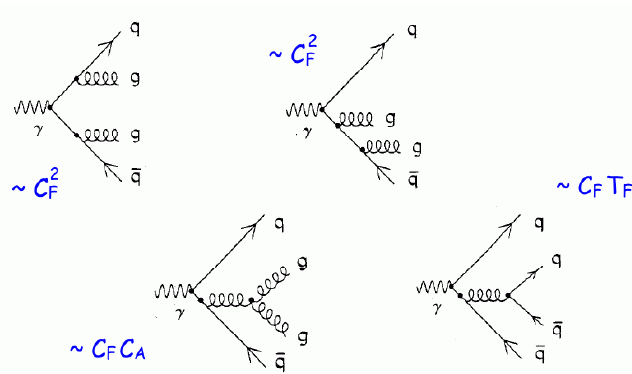
\includegraphics[width=0.8\linewidth]{QCD/4jets.png}
    \caption{Mogelijke diagrammen om 4 jets te maken}%
    \label{fig:4jets}
\end{figure}

Hiervan is de eerste jet heel makkelijk te onderscheiden van de andere 3 vanwege zijn topologie. De eerste heeft 2 jets die in de ene richting zullen gaan en 2 jets in de andere richting. De andere 3 configuraties hebben 1 jet die met ongeveer de helft van de impuls in de ene richting zal gaan en de overige 3 jets die in de andere richting gaan. Wat er gebeurt in deze diagrammen kan gereduceerd worden tot 3 verschillende processen.

\begin{figure}[h]
    \centering
    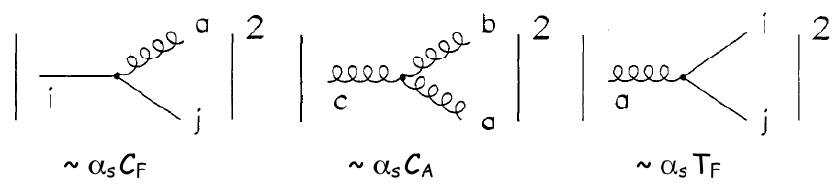
\includegraphics[width=0.8\linewidth]{QCD/reduced_events.png}
    \caption{Gereduceerde diagram elementen}%
    \label{fig:reduced_events}
\end{figure}

Deze zijn evenredig met de sterke koppelingsconstante en de kleurfactoren $C_F$, $C_A$ en $T_F$. Deze kleurfactoren zijn niets anders dan het aantal kleurcombinaties dat er mogelijk zijn. Het is makkelijk in te zien dat die factoren zich ook zullen tonen in de verschillende mogelijkheden om 4 jets te creëren. Dit kunnen we gebruiken om de symmetrieën tussen de kleuren onderzoeken. De kinematica van deze experimenten hangt dus af van de diagrammen. Als we hier nu $C_A/C_F$ en $T_F/C_F$ bepalen, kunnen we de groepen van de kleuren bepalen.

\begin{table}[h]
    \centering
    \caption{Symmetrie van de kleurconstantes}
    \label{tab:sym_kleurfact}
    \begin{tabular}{|c|c|c|c|}
        \hline
        Groep   & $C_A$ & $C_F$         & $T_F$ \\
        \hline
        $SU(3)$ & 3     & 4/3           & 1/2   \\
        $U(1)_3$& 0     & 1             & 3     \\
        $SO(3)$ & 3     & 3             & 3     \\
        $SU(N)$ & $N$   & $(N^2-1)/2N$  & 1/2   \\
        \hline
    \end{tabular}
\end{table}

In tabel \ref{tab:sym_kleurfact} kan je de waarden terug vinden voor de kleurfactoren indien QCD een bepaalde groep zou hebben. Uit dit experiment, zoals bij het LEP (figuur \ref{fig:4jets_results}), zien we dat het een goede aanname was dat we hiervoor $SU(3)$ gebruiken.

\begin{figure}[h]
    \centering
    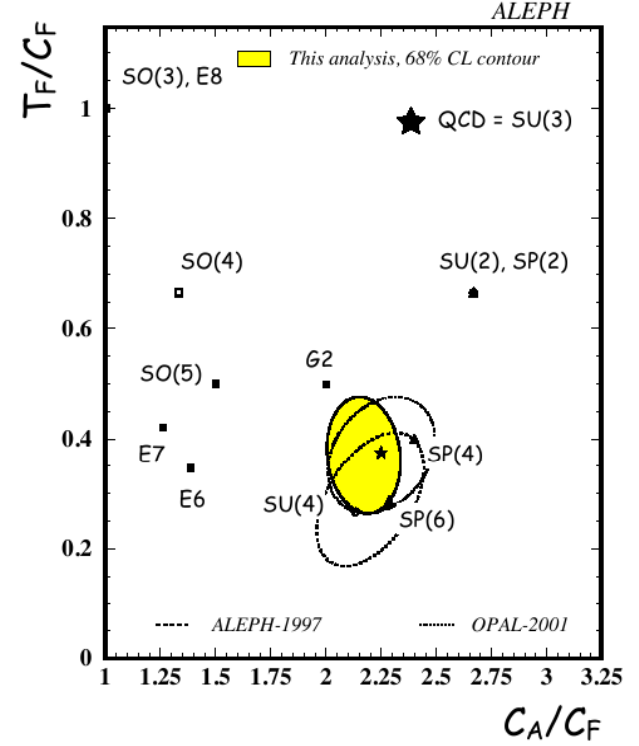
\includegraphics[width=0.4\linewidth]{QCD/4jets_results.png}
    \caption{Lep resultaten voor 4 jet experimenten}%
    \label{fig:4jets_results}
\end{figure}

{\color{red} Wat Ryckbosch vooral interessant vindt hier, is dat je weet waarom $C_A$ bij $U(1)_3$ 0 is. Dit komt omdat $U(1)$ een abelse groep is en zelfinteractie niet mogelijk is.}

\subsection{Spin van het gluon}%
\label{sub:spin_van_het_gluon}

\begin{figure}[h]
    \centering
    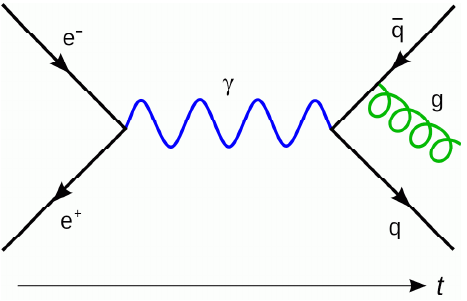
\includegraphics[width=0.4\linewidth]{QCD/3jets.png}
    \caption{3 jet evenementen}%
    \label{fig:3jets}
\end{figure}

Hier drijven we de experimenten nog een beetje verder en kijken we naar 3-jet evenementen. In deze experimenten maken we weer een quark-antiquark paar aan waarvan er 1 een gluon afstraalt. Hier zal een spin $1/2$ deeltje een vector boson met spin $1$ aanmaken. Het behoud van angulair moment zorgt ervoor dat de hoekdistributie afhangt van het feit of het gluon nu een spin 0 of spin 1 deeltje is.
Bij deze experimenten zoek je de jet met de hoogste energie, die waarschijnlijk degene is die niets heeft afgestraald. Dan kan je kijken naar de hoekdistributie tussen de andere 2 en kan je een idee krijgen over de spin van het gluon. In de resultaten van deze experimenten (figuur \ref{fig:3jets_results}) zien we dat deze de curve zal beschrijven voor een spin 1 deeltje en is het gluon dus een vector gluon.

\begin{figure}[h]
    \centering
    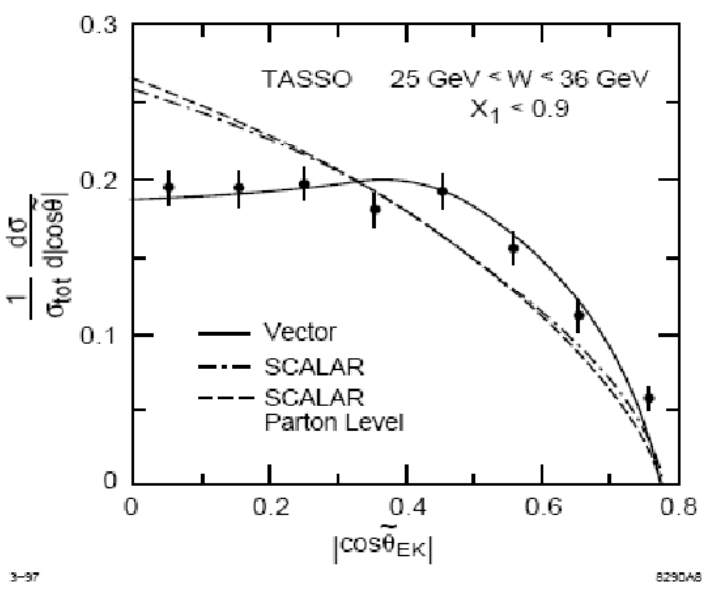
\includegraphics[width=0.8\linewidth]{QCD/3jets_results.png}
    \caption{Onderzoek naar de spin van het gluon}%
    \label{fig:3jets_results}
\end{figure}

\subsection{$\alpha_s$}%
\label{sub:_alpha_s_}

Wat we al hebben gezien is de sterke koppelingsconstante bij de massa van het $Z$ boson (figuur \ref{fig:str_kop_z}).

\begin{figure}[h]
    \centering
    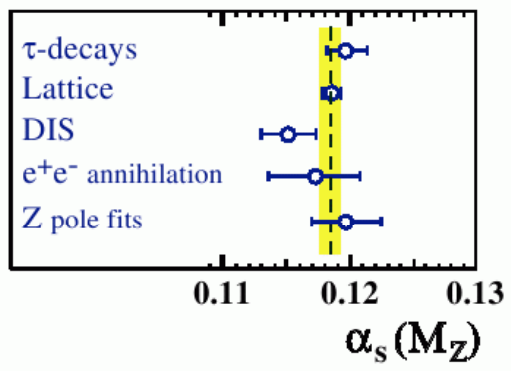
\includegraphics[width=0.8\linewidth]{QCD/str_kop_z.png}
    \caption{De sterke koppelingsconstante bij de massa van het $Z$ boson}%
    \label{fig:str_kop_z}
\end{figure}

Indien we dit voor meerdere massa's en verschillende energieën uitvoeren krijgen we uiteindelijk te zien dat de waarde van de sterke koppelingsconstante zal oplopen (figuur \ref{fig:running_str_kop}).

\begin{figure}[h]
    \centering
    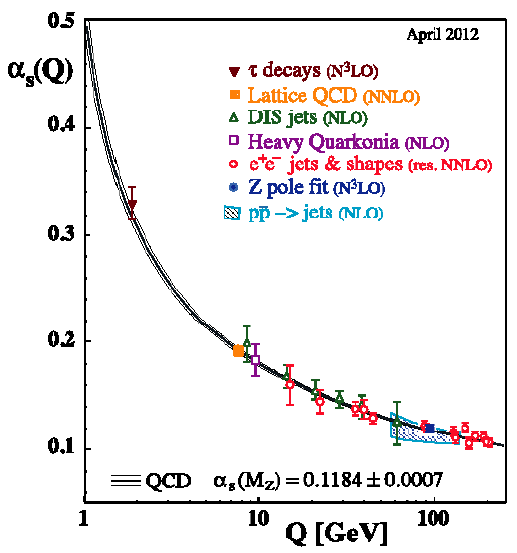
\includegraphics[width=0.6\linewidth]{QCD/running_str_kop.png}
    \caption{Lopende koppelingsconstante}%
    \label{fig:running_str_kop}
\end{figure}

Het interessante bij deze grafiek is dat de meest accurate metingen voor QCD komen uit het onderzoek van een zwakke interactie. Hierbij is de vorm van de curve bepaald door QCD en gefit aan de waarde van het $Z$ boson.

\subsection{Lopende koppelingsconstante}%
\label{sub:lopende_koppelingsconstante}

\subsubsection{QED}%
\label{ssub:qed}

Bij QED wordt de effectieve lading van het elektron bepaald door het proces:\\
\begin{minipage}[c]{0.5\textwidth}
    \begin{center}
        \feynmandiagram[inline=(a), horizontal=b to c]{
            a -- [photon, edge label=\(\gamma\)] b,
            i1 -- [fermion] a,
            a -- [fermion] i2,
            f1 -- [fermion] b,
            b -- [fermion] f2,
        };
    \end{center}
    \begin{equation}
        \begin{aligned}
            \label{eq:QED_eerste_orde}
            P_0 = \frac{e_0^2}{q^2}
        \end{aligned}
    \end{equation}
\end{minipage}\noindent
\begin{minipage}[c]{0.5\textwidth}
    \begin{center}
        \feynmandiagram[inline=(a), horizontal=a to b]{
            a -- [photon, edge label=\(\gamma\)] b
            -- [fermion, half left, looseness=1.5] c
            -- [fermion, half left, looseness=1.5] b,
            c -- [photon, edge label=\(\gamma\)] d,
            i1 -- [fermion] a,
            a -- [fermion] i2,
            f1 -- [fermion] d,
            d -- [fermion] f2,
        };
    \end{center}
    \begin{equation}
        \begin{aligned}
            \label{eq:QED_tweede_orde}
            P = P_0\pi(q^2)P_0
        \end{aligned}
    \end{equation}
\end{minipage}
Uiteindelijk krijgen voor alle ordes samen dat:
\begin{equation}
    \begin{aligned}
        \label{eq:QED_all}
        p&=P_0\pi(q^2)P_0+P_0\pi(q^2)\pi(q^2)P_0+...\\
         &=P_0 \frac{1}{1-\pi(q^2)P_0} \\
         &=P_0 \frac{1}{1-e_0^2\prod(q^2)} 
    \end{aligned}
\end{equation}
Hierbij hebben we gebruik gemaakt van Taylor ontwikkelingen waarbij x natuurlijk kleiner moet zijn dan 1. Bij de laatste gelijkheid hebben we een zelfenergiecorrectie geïsoleerd waar de lading uit is gehaald. We zien dus dat een foton omgeven zal zijn door een wolk van deeltje-antideeltje paren die hij zal aanmaken en opslorpen. We kunnen de lading van het elektron nu schrijven als de lading bij het eerste diagram vermenigvuldigd met de uitkomst uit vergelijking (\ref{eq:QED_all}).
\begin{equation}
    \begin{aligned}
        \label{eq:running_lading}
        e^2(q^2) = \frac{e_0^2}{1-e_0^2\prod(q^2)} 
    \end{aligned}
\end{equation}
De effectieve lading hangt dus af van op welke afstand we er gaan naar kijken. Schalen we dit nu naar $\mu$, een basisschaal, dan krijgen we
\begin{equation}
    \begin{aligned}
        \label{eq:running_lading_1}
        e^2(\mu^2) = \frac{e_0^2}{1-e_0^2\prod(\mu^2)} 
    \end{aligned}
\end{equation}
Zo bekomen we dat de elementaire lading gegeven kan worden door
\begin{equation}
    \begin{aligned}
        \label{eq:running_lading_2}
        e_0^2 &= \frac{e^2(\mu^2)}{1-e^2(\mu^2)\prod(\mu^2)} \\
        e^2(q^2) &= \frac{e^2(\mu^2)}{1-e^2(\mu^2)\cdot [\prod(q^2)-\prod(\mu^2)]}
    \end{aligned}
\end{equation}
Het enige dat loopt in deze vergelijking is de $\prod{q^2}$ term. Het is mogelijk om in QCD $\prod(q^2)-\prod(\mu^2)$ uit te rekenen. Hiervoor wordt er verwezen naar het vak kwantumveldentheorie. Hetgeen we hier hebben is eigenlijk niets anders dan de EM koppelingsconstante
\begin{equation}
    \begin{aligned}
        \label{eq:em_koppelingsconstante}
        \alpha(q^2) &= \frac{\alpha(\mu^2)}{1-\alpha(\mu^2) \frac{1}{3\pi} ln\left( \frac{q^2}{\mu^2} \right)}
    \end{aligned}
\end{equation}
Dit is wat we ook zullen waarnemen bij hoge energieën, maar niet wat we gebruiken in het dagelijkse leven. Daar is $\alpha = \frac{1}{137}$. We zien dat bij hogere energieën de elektrische lading sterker zal worden. Dit omdat als we naar zo kleine afstanden van enkele fm beginnen te kijken, er een nieuw fenomeen begint te spelen. Een lading zal voortdurend fotonen afstralen en in lading-antilading paren omgaan. Het positieve gedeelte van het paar wordt gericht naar de negatieve lading. Met andere woorden wordt het vacuum rond de lading gepolariseerd. Het moment dat we binnen dat gepolariseerde gebied beginnen te kijken zien we die shields van de gepolariseerde lading niet meer en zullen we de echte lading van het deeltje beginnen zien.

\subsubsection{QCD}%
\label{ssub:qcd}

Deze zelfde denkwijze kunnen we nu toepassen op QCD. We krijgen naast de equivalente diagrammen in QED ook nog andere mogelijkheden. In eerste orde hebben we nu:\\
\begin{minipage}[c]{0.3\textwidth}
    \begin{center}
        \feynmandiagram[inline=(a), horizontal=a to b]{
            a -- [gluon] b
            -- [fermion, half left, looseness=1.5] c
            -- [fermion, half left, looseness=1.5] b,
            c -- [gluon] d,
            i1 -- [fermion] a,
            a -- [fermion] i2,
            f1 -- [fermion] d,
            d -- [fermion] f2,
        };
    \end{center}
\end{minipage}\noindent
\begin{minipage}[c]{0.3\textwidth}
    \begin{center}
        \feynmandiagram[inline=(a), horizontal=a to b]{
            a -- [gluon] b
            -- [gluon, half left, looseness=1.5] c
            -- [gluon, half left, looseness=1.5] b,
            c -- [gluon] d,
            i1 -- [fermion] a,
            a -- [fermion] i2,
            f1 -- [fermion] d,
            d -- [fermion] f2,
        };
    \end{center}
\end{minipage}\noindent
\begin{minipage}[c]{0.3\textwidth}
    \begin{center}
        \feynmandiagram[inline=(a), horizontal=a to d]{
            a -- [gluon] b,
            b -- [gluon, half left] c;
            c -- [gluon, half left] b,
            b -- [gluon] d,
            i1 -- [fermion] a,
            a -- [fermion] i2,
            f1 -- [fermion] d,
            d -- [fermion] f2,
        };
    \end{center}
\end{minipage}\\
Nog een andere mogelijkheid is
\begin{center}
    \feynmandiagram [small, horizontal=a to t1] {
        i1 -- a -- i2,
        a -- [gluon] t1 -- [gluon] t2 -- t3 -- [gluon] t1,
        t2 -- p1,
        t3 -- p2,
    };
\end{center}
Het resultaat voor de lopende sterke koppelingsconstante zal  naast deze extra diagrammen ook nog afhangen van het aantal flavours $n_f$ en het aantal kleuren $n_c$. Zo krijgen we
\begin{equation}
    \begin{aligned}
        \label{eq:running_strong}
        \alpha_s(q^2) = \frac{\alpha_s(\mu^2)}{1+\alpha_s(\mu^2) \frac{11n_c-2n_f}{12\pi} \ln\left(\frac{q^2}{\mu^2}\right)} 
    \end{aligned}
\end{equation}
 Hier zal een belangrijke eigenschap bovenkomen. Vanaf het moment dat $11n_c>2n_f$, zal de noemer altijd maar groter worden met grotere q waarden en wordt de sterke koppelingsconstante steeds kleiner als we op kleinere afstanden kijken. De reden voor deze verzwakking is juist hetzelfde als bij het elektron. De quark straalt terug gluonen uit die quark-antiquark paren zal maken. Zo hebben we rond de quark een wolk van quark-antiquark paren die het vacuum rond de quark polariseren. Het verschil hier is dat gluonen zelf kleur hebben en kleur zullen wegnemen van de quark. Hoe dichter je dus bij de quark komt, hoe meer kleur is weggestraald en hoe minder kleur je zal waarnemen en hoe kleiner de koppeling zal worden. De factor waarmee kleur zal weggenomen worden door QCD is:
\begin{equation}
    \begin{aligned}
        \label{eq:kleur_qcd}
        \lambda_{QCD} \equiv \mu \exp(-12\pi/(33-2n_f)\alpha_s(\mu^2))
    \end{aligned}
\end{equation}
Dit alles noemen we de asymptotische vrijheid. Eens de quarks zo dicht bij elkaar zijn, zullen ze elkaar niet meer voelen. Omgekeerd, als een quark en een antiquark van elkaar weggaan, trekken ze elkaar meer aan. Dit effect noemen we fluxbuizen. Typische schalen zijn hier terug $1GeV/fm$. Wat zijn de gevolgen nu van deze opsluiting?

\subsection{DIS: scaling violations}%
\label{sub:dis_scaling_violations}

Het meest spectaculaire gedeelte van deze opsluiting kunnen we zien in de scaling violations die we waarnemen. Initieel keken we enkel naar de diep inelastische verstrooiingen bij brave energieën van $1-10GeV^2$. Volgens deze experimenten was er geen afhankelijkheid van de $F_2$ in functie van $Q^2$ en werd bewezen dat dit puntdeeltjes waren. Het moment dat we over een veel grotere range kijken, zie figuur \ref{fig:scale_viol}, zien we dat hier toch een grote variatie aanwezig is. We zien dat bij lage $x$ de waarschijnlijkheid om een quark waar te nemen afneemt met hogere $Q^2$ en voor grote $x$ zal toenemen met hogere $Q^2$. De reden hiervoor is een resolutie-effect (figuur \ref{fig:dis_resolutie}). Als een laagenergetisch foton interageert, ziet hij een puntlading waarmee hij zal interageren. Als met hoogenergetische fotonen wordt gekeken naar een hadron zien ze nog steeds een puntdeeltje, maar een dat kleiner is en dat de mogelijkheid heeft gehad om een gluon af te stralen $\rightarrow$ de quark heeft een kleinere impuls fractie dan de originele quark. \hl{Bij verhogende energieën is het steeds minder waarschijnlijk om een quark met een hoge impulsfractie tegen te komen.}

\begin{figure}[h]
    \centering
    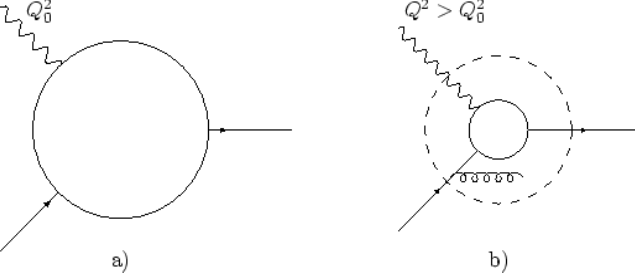
\includegraphics[width=0.8\linewidth]{QCD/resolutie.png}
    \caption{Resolutie effect bij DIS experimenten}%
    \label{fig:dis_resolutie}
\end{figure}

\subsection{Splitting functies}%
\label{sub:splitting_functies}

\begin{wrapfigure}[9]{l}{0.25\textwidth}
    \centering
    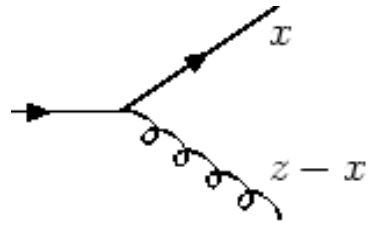
\includegraphics[width=0.9\linewidth]{QCD/split_func.png}
    \caption{diagram van splitting functies}
    \label{fig:split_func}
\end{wrapfigure}
In QCD is het mogelijk om deze afsplitsing verder uit te werken. Dit zijn de zogenaamde splitting functies. Die geven de waarschijnlijkheid om een quark met impulsfractie $z$ op te splitsen in een quark met impulsfractie $x$ en een gluon met fractie $z-x$.
\begin{equation}
    \begin{aligned}
        \label{eq:split_func}
        q(z)\rightarrow q(x) + g(z-x)
    \end{aligned}
\end{equation}
Omdat in dit diagram een vertex aanwezig is, is er natuurlijk een afhankelijkheid van $\alpha_s$ aanwezig. De kleurfactor $C_F$ is hier ook aanwezig. Naast het splitsen van het momentum over partons gegeven in vergelijking (\ref{eq:split_func}) zijn er nog andere manieren om dit momentum op te splitsen:
\begin{equation}
    \begin{aligned}
        \label{eq:split_func_all}
        q(z)&\rightarrow q(x) + g(z-x)\\
        q(z)&\rightarrow g(x) + q(z-x)\\
        g(z)&\rightarrow g(x) + g(z-x)\\
        g(z)&\rightarrow q(x) + \overline q(z-x)
    \end{aligned}
\end{equation}
Bij deze verschillende manieren van opsplitsen zal natuurlijk ook gebruik gemaakt worden van de andere kleurfactoren.\\
Bij schaalbreking worden we dus uiteindelijk ook gevoelig voor de gluondistributies omdat deze ook weer quarks en antiquarks kunnen aanmaken.

\begin{figure}[h]
    \centering
    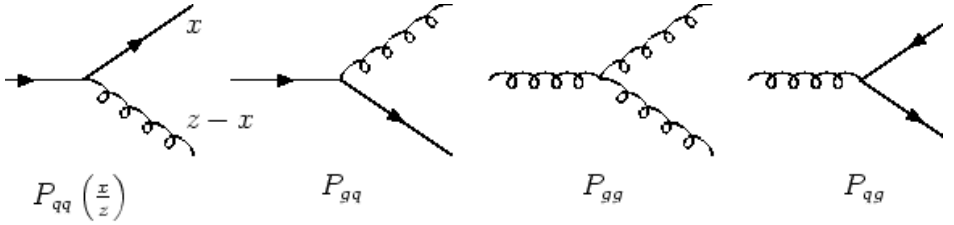
\includegraphics[width=0.8\linewidth]{QCD/split_func_all.png}
    \caption{diagrammen van alle split mogelijkheden}%
    \label{fig:split_func_all}
\end{figure}

Uit berekeningen in QCD krijgen we nu de verschillende mogelijkheden om een soort van splitsing tegen te komen:
\begin{equation}
    \begin{aligned}
        \label{eq:}
        P_{qq}(Z) &= \frac{4}{3} \frac{1+Z^2}{1-Z} \\
        P_{gq}(Z) &= \frac{4}{3} \frac{1+(1-Z)^2}{Z} \\
        P_{gg}(Z) &= 6 \left( \frac{1-Z}{Z} + \frac{Z}{1-Z} + Z(1-Z) \right) \\
        P_{qg}(Z) &= \frac{1}{2} \left( Z^2 + (1-Z)^2 \right) \\
    \end{aligned}
\end{equation}
met $Z= \frac{x}{z}$. Een belangrijke opmerking bij de laatste 2 diagrammen is dat de uitgaande deeltjes perfeect symmetrisch moeten zijn met elkaar. Dit kunnen we natuurlijk ook zien in hun vergelijkingen die symmetrisch zijn voor $Z$ en $1-Z$. Misschien een minder interessante opmerking, maar zeker niet onopgemerkt: voor de eerste waarschijnlijkheid zien we dat als de quark zo goed als alle impuls krijgt, dat deze waarschijnlijkheid afneemt. Dit is uiteindelijk logisch omdat een laagenergetisch gluon lange afstanden zou afleggen, wat onmogelijk is in QCD. De equivalenten gebeuren natuurlijk ook in de andere waarschijnlijkheden.

\subsection{DGLAP}%
\label{sub:dglap}

De verschillende waarschijnlijkheids distributies om te veranderen in quarks, antiquarks of gluons kunnen nu gegeven worden door:
\begin{equation}
    \begin{aligned}
        \label{eq:dglap}
        Q^2 \frac{dq_i(x, Q^2)}{dQ^2} = \frac{dq_i(x,Q^2)}{d\ln Q^2} &= \frac{\alpha_s}{2\pi} \int_x^1 \frac{dz}{z} \left[ q_i(z,Q^2)P_{qq}\left( \frac{x}{z} \right) + g(z,Q^2)P_{qg} \left( \frac{x}{z} \right) \right]\\
        Q^2 \frac{d\overline q_i(x, Q^2)}{dQ^2} = \frac{d\overline q_i(x,Q^2)}{d\ln Q^2} &= \frac{\alpha_s}{2\pi} \int_x^1 \frac{dz}{z} \left[ \overline q_i(z,Q^2)P_{qq}\left( \frac{x}{z} \right) + g(z,Q^2)P_{qg} \left( \frac{x}{z} \right) \right]\\
        Q^2 \frac{dg_i(x, Q^2)}{dQ^2} = \frac{dg_i(x,Q^2)}{d\ln Q^2} &= \frac{\alpha_s}{2\pi} \int_x^1 \frac{dz}{z} \left[ \sum_i q_i(z,Q^2)P_{gq}\left( \frac{x}{z} \right) + \sum_i \overline q_i(z,Q^2)P_{gq}\left( \frac{x}{z} \right) + g(z,Q^2)P_{gg} \left( \frac{x}{z} \right) \right]\\
    \end{aligned}
\end{equation}
{\color{green} Opmerking: De $\alpha_s$ in deze vergelijkingen is nog steeds afhankelijk van $Q^2$.}
Deze vergelijkingen kan je nu fitten aan wat we in de experimenten hebben gevonden en we zien dat deze theorie de experimenten zo goed als perfect kan volgen. Het probleem dat we hebben met QCD met de grote afstanden zal in de DGLAP vergelijkingen weggeintegreerd worden.

\subsection{Hadron colliders}%
\label{sub:hadron_colliders}

De parton distributie functies zullen hier heel belangrijk zijn omdat hier niet echt de hadronen zullen verstrooiien met elkaar maar eerder de partons.
\begin{equation}
    \begin{aligned}
        \label{eq:hadr_coll}
        A+B &\rightarrow C + R\\
        \text{parton level: } a+b&\rightarrow c+r
    \end{aligned}
\end{equation}
De uiteindelijke cross sectie van deze verstrooiing is gegeven door:
\begin{equation}
    \begin{aligned}
        \label{eq:hadr_coll_cross_sec}
        \sigma(AB\rightarrow CR) = \int dx_a \int dx_b \left[ \left[ f_{a/A}(x_a) f_{b/B}(x_b) + f_{a/B}(x_a) f_{b/B}(x_b) \right] \times \sigma(ab\rightarrow cr,\hat s)\right]
    \end{aligned}
\end{equation}
met $f_{...}$ de parton distributie functies die moeten gemeten worden. Er zijn meerdere diagrammen die kunnen bijdragen in de hadronverstrooiingen.

\begin{figure}[h]
    \centering
    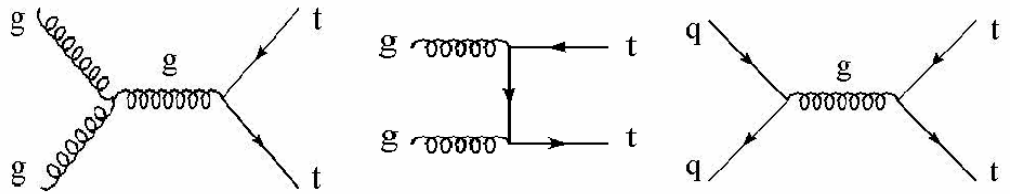
\includegraphics[width=0.8\linewidth]{QCD/hadr_coll_diagr.png}
    \caption{Diagrammen in de hadron collisies}%
    \label{fig:QCD/hadr_coll_diagr}
\end{figure}

Uit de parton distributiefuncties (figuur \ref{fig:part_dist_func}) kunnen we ook zien dat bij de hogere energieën het meer en meer waarschijnlijk zal zijn dat er verstrooid wordt aan een gluon in plaats van een (anti)quark. Als 2 voorbeelden hebben we de Tevatron en de LHC. De Tevatron werkt bij ongeveer 1TeV en bestaat voor 80\% uit het annihileren van een quark-antiquark paar tot een gluon en maar 20\% uit gluon fusies. Daarentegen werkt de LHC bij 10TeV en bestaat uit 80\% gluon fusies en 20\% quark paar annihilaties.

\end{document}
